%%%%%%%%%%%%%%%%%%%%%%%%%%%%%%%%%%%%%%%%%
% Stylish Article
% LaTeX Template
% Version 2.2 (2020-10-22)
%
% This template has been downloaded from:
% http://www.LaTeXTemplates.com
%
% Original author:
% Mathias Legrand (legrand.mathias@gmail.com) 
% With extensive modifications by:
% Vel (vel@latextemplates.com)
%
% License:
% CC BY-NC-SA 3.0 (http://creativecommons.org/licenses/by-nc-sa/3.0/)
%
%%%%%%%%%%%%%%%%%%%%%%%%%%%%%%%%%%%%%%%%%

%----------------------------------------------------------------------------------------
%	PACKAGES AND OTHER DOCUMENT CONFIGURATIONS
%----------------------------------------------------------------------------------------

\documentclass[fleqn,10pt]{SelfArx} % Document font size and equations flushed left

\usepackage[english]{babel} % Specify a different language here - english by default

\usepackage{lipsum,cite} % Required to insert dummy text. To be removed otherwise

%----------------------------------------------------------------------------------------
%	COLUMNS
%----------------------------------------------------------------------------------------

\setlength{\columnsep}{0.55cm} % Distance between the two columns of text
\setlength{\fboxrule}{0.75pt} % Width of the border around the abstract

%----------------------------------------------------------------------------------------
%	COLORS
%----------------------------------------------------------------------------------------

\definecolor{color1}{RGB}{0,0,90} % Color of the article title and sections
\definecolor{color2}{RGB}{0,20,20} % Color of the boxes behind the abstract and headings

%----------------------------------------------------------------------------------------
%	HYPERLINKS
%----------------------------------------------------------------------------------------

\usepackage{hyperref} % Required for hyperlinks

\hypersetup{
	hidelinks,
	colorlinks,
	breaklinks=true,
	urlcolor=color2,
	citecolor=color1,
	linkcolor=color1,
	bookmarksopen=false,
	pdftitle={Title},
	pdfauthor={Author},
}

%----------------------------------------------------------------------------------------
%	ARTICLE INFORMATION
%----------------------------------------------------------------------------------------

\JournalInfo{Survey Report, 7, Nov, 2024} % Journal information
\Archive{Final report for AI3605} % Additional notes (e.g. copyright, DOI, review/research article)

\PaperTitle{Opportunities and Challenges of Large Language Models in Industry Applications} % Article title

\Authors{Yuan Gao}
% \Authors{John Smith\textsuperscript{1}} % Authors
% \affiliation{\textsuperscript{1}\textit{}} % Author affiliation



\Keywords{Keyword1 --- Keyword2 --- Keyword3} % Keywords - if you don't want any simply remove all the text between the curly brackets
\newcommand{\keywordname}{Keywords} % Defines the keywords heading name

%----------------------------------------------------------------------------------------
%	ABSTRACT
%----------------------------------------------------------------------------------------

\Abstract{
	In recent years, large language models(LLMs) have gained gained significant attention not only in academic, but also in industry. With the rising demand of the LLMs and the incredible potential interest of the AI-powered applications, it occurs massive opportunities also challenges. These LLMs, including GPT-4, Gemini, Qwen, and other advanced models, have demonstrated there abilities to automate tasks such as writing, coding, analysis and more. They are also transforming fields like healthcare, education, marketing by enabling prominent personalization and efficiency. However, there still exists several challenges performing as obstacles to the development of LLMs, including data privacy, ethics, cost and more. In this survey, we will explore and discuss about both opportunities and chanllenges of LLMs in industrial applications, providing insights into current research and future directions for addressing these obstacles.
}

%----------------------------------------------------------------------------------------



\begin{document}

\maketitle % Output the title and abstract box

\tableofcontents % Output the contents section

\thispagestyle{empty} % Removes page numbering from the first page

%----------------------------------------------------------------------------------------
%	ARTICLE CONTENTS
%----------------------------------------------------------------------------------------

\section*{Introduction} % The \section*{} command stops section numbering

\addcontentsline{toc}{section}{Introduction} % Adds this section to the table of contents

% paragraph 1 : Briefly introduce the concept and background of large language models (LLMs)

% paragraph 2 : Explain the importance and influence of LLMs in the field of artificial intelligence

% paragraph 3 : Outline the objectives and structure of the report

% \lipsum[1-3] % Dummy text
%  and some mathematics $\cos\pi=-1$ and $\alpha$ in the text\footnote{And some mathematics $\cos\pi=-1$ and $\alpha$ in the text.}.

The field of natural language processing (NLP) has changed a lot with the rise of large language models (LLMs). Coming from years of research in computational linguistics and deep learning, LLMs are based on early work like the use of neural networks for language modeling in the late 1990s and the transformer-based architectures introduced by Vaswani et al. \cite{Vaswani:2017at}. These steps led to the creation of models like GPT \cite{Radford:2018tf}, BERT \cite{Devlin:2018br}, and, more recently, GPT-4, Gemini, and Qwen, which now surpass humans in many language tasks.

In the beginning, LLMs were praised in academic settings for advancing research in linguistics and machine learning. Their uses were mostly experimental, focusing on benchmarks and competitions like GLUE and SuperGLUE. But as models grew larger and AI-powered tools became more common, their use spread beyond academia. Now, industries like healthcare and marketing use LLMs to transform their work. These models help automate tasks like creating content, programming, and making decisions.

\begin{figure}[ht]\centering
	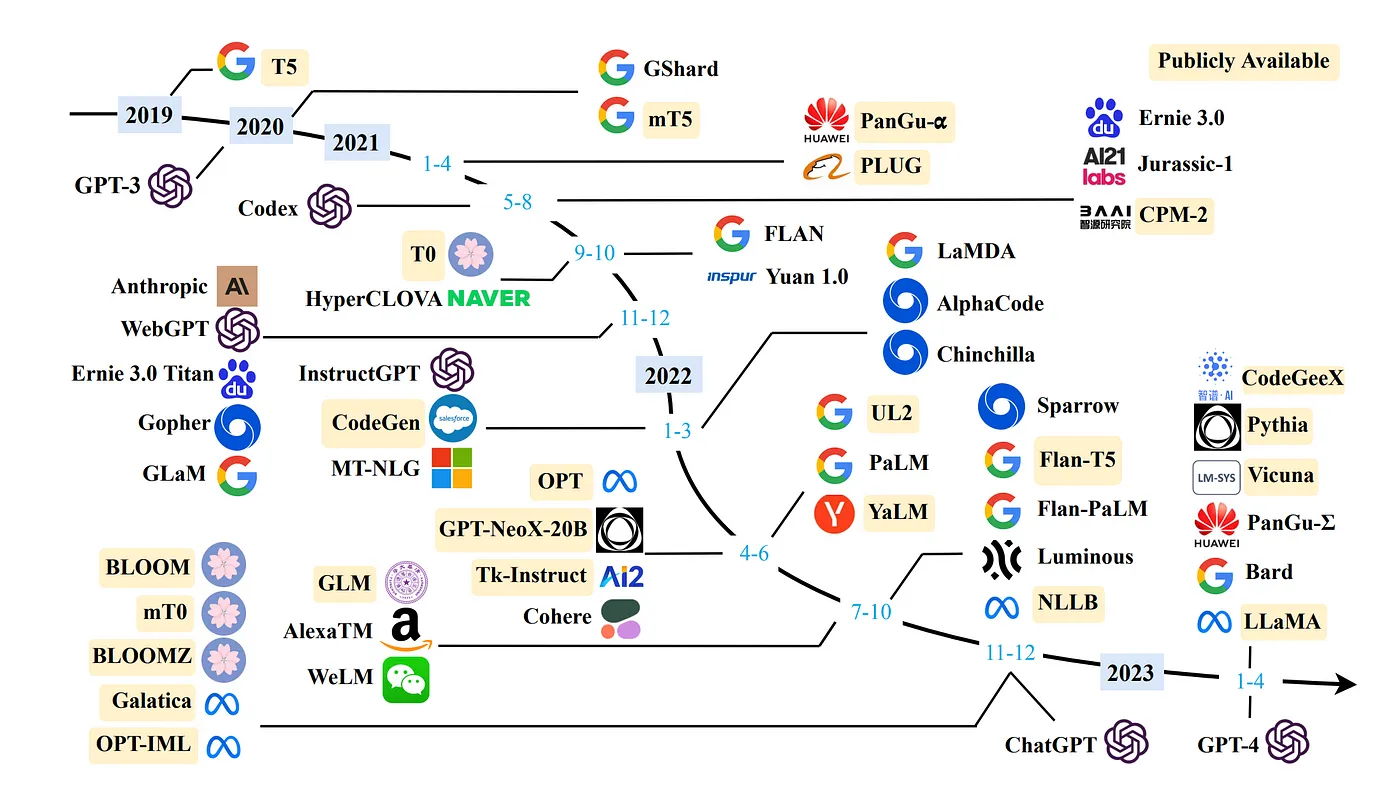
\includegraphics[width=\linewidth]{Figures/development.png}
	\caption{Chronological development of large language models (LLMs) from 2019 to 2023.}
	\label{fig:dev}
\end{figure}

After the coming of GPT-3, the whole industry make sense that the era of LLMs are coming. From 2020 to now, industry release their LLMs like mushrooms after rain, few of them make a significant success including Claude, Gemini, Ernie, LLaMA. While others are still trying their best to make their LLMs outstanding. We can briefly grasp the development context by Figure\ref{fig:dev}

Even with their promise, using LLMs in industries comes with challenges. Problems like data privacy, ethical concerns, and the high cost of running these models often slow their wider use \cite{Bender:2021ai}. These issues not only limit their usefulness but also show gaps in research and implementation.

This survey aims to connect advances in research with real-world applications of LLMs. By collecting input from professionals and researchers, the study looks to find ways to use LLMs better in industries while addressing the problems that hold them back. The results aim to add to the discussion about AI’s role in society and offer useful ideas for researchers, policymakers, and business leaders.

%------------------------------------------------

\section{Overview of Core-tech in LLMs}

% \begin{figure*}[ht]\centering % Using \begin{figure*} makes the figure take up the entire width of the page
% 	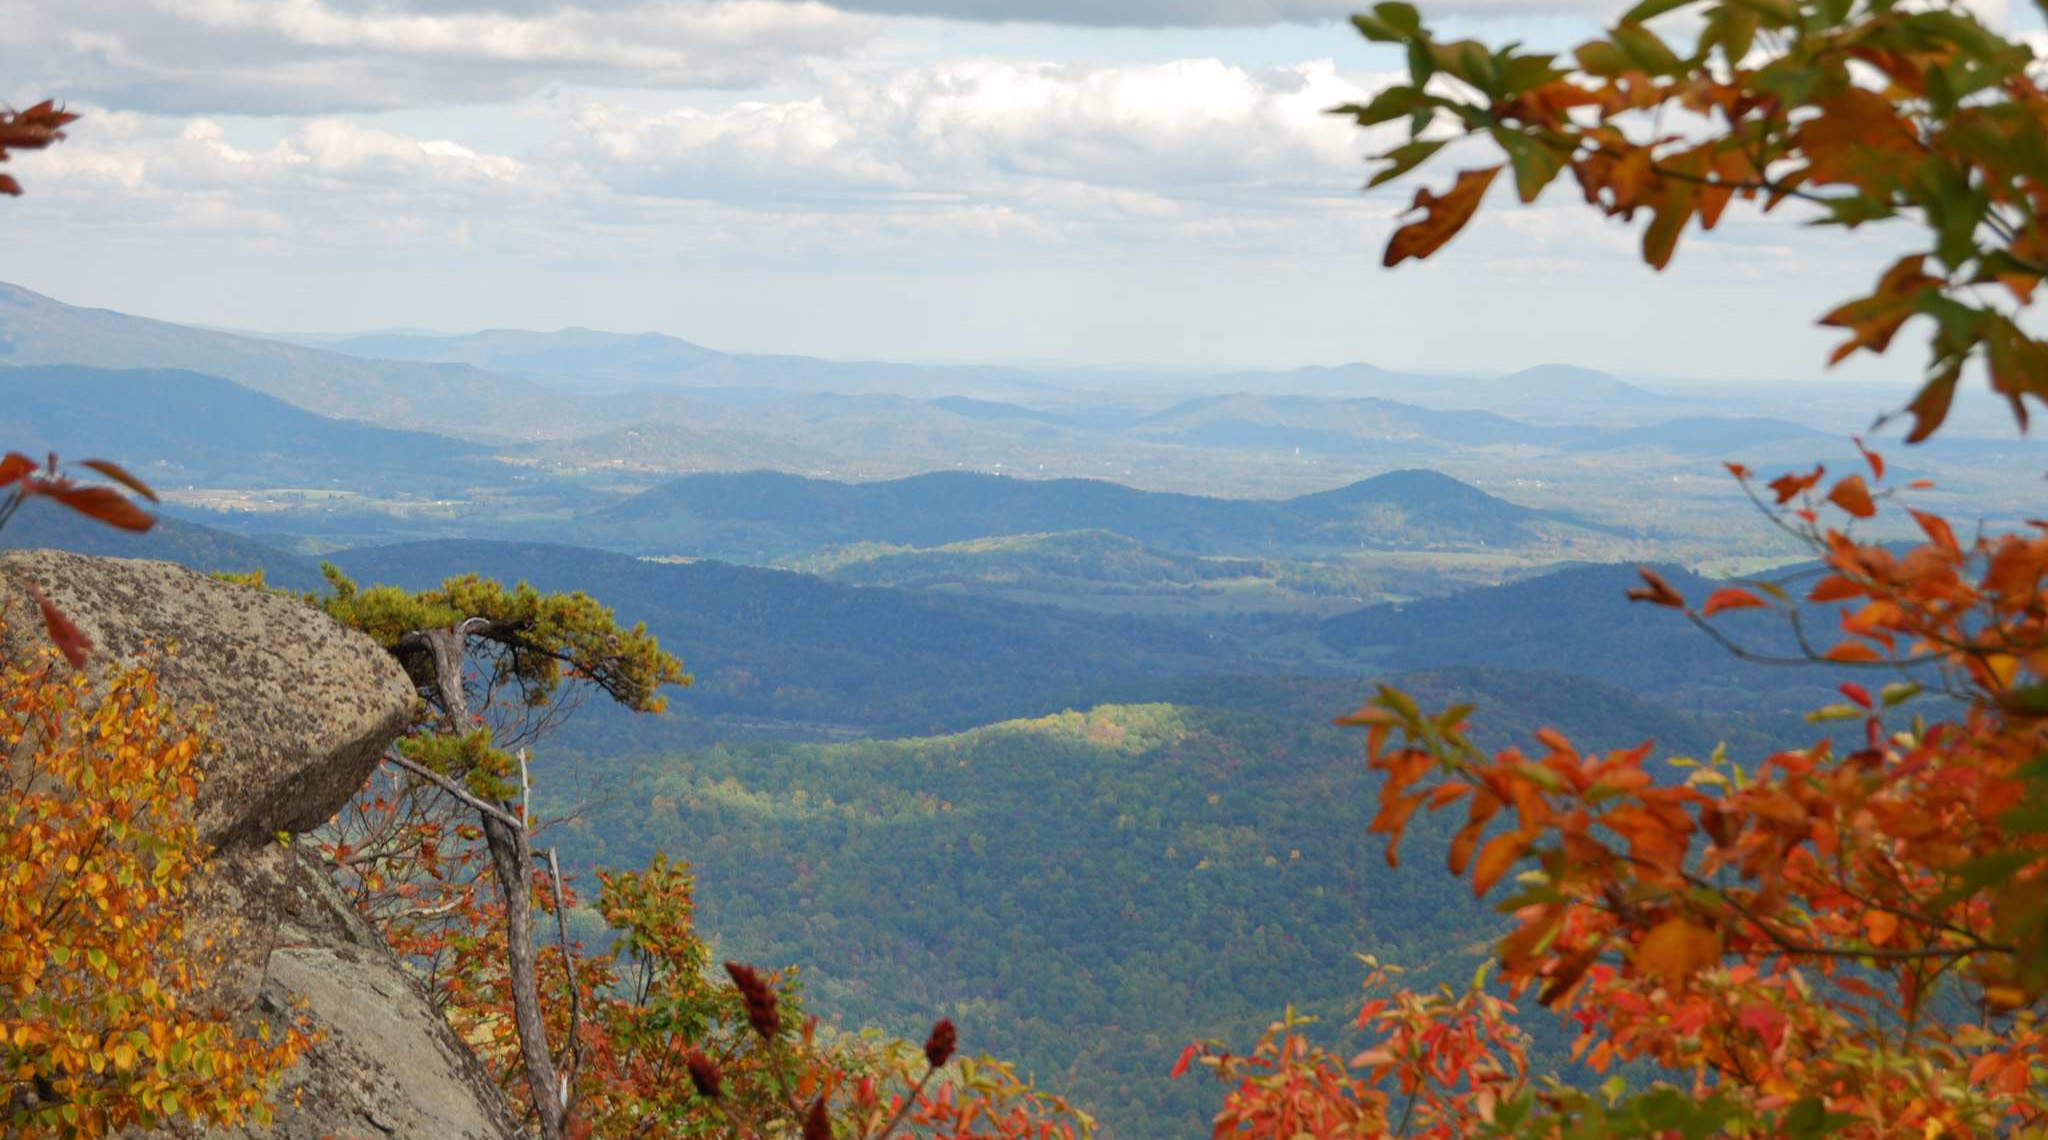
\includegraphics[width=\linewidth]{view}
% 	\caption{Wide Picture}
% 	\label{fig:view}
% \end{figure*}

% \lipsum[4] % Dummy text

% \begin{equation}
% 	\cos^3 \theta =\frac{1}{4}\cos\theta+\frac{3}{4}\cos 3\theta
% 	\label{eq:refname2}
% \end{equation}

% \lipsum[5] % Dummy text

% \begin{enumerate}[noitemsep] % [noitemsep] removes whitespace between the items for a compact look
% 	\item First item in a list
% 	\item Second item in a list
% 	\item Third item in a list
% \end{enumerate}

\subsection{Machanism}

% \lipsum[6] % Dummy text

\paragraph{Paragraph} \lipsum[7] % Dummy text
\paragraph{Paragraph} \lipsum[8] % Dummy text

\subsection{Architectures}

% \lipsum[9] % Dummy text

% \begin{figure}[ht]\centering
% 	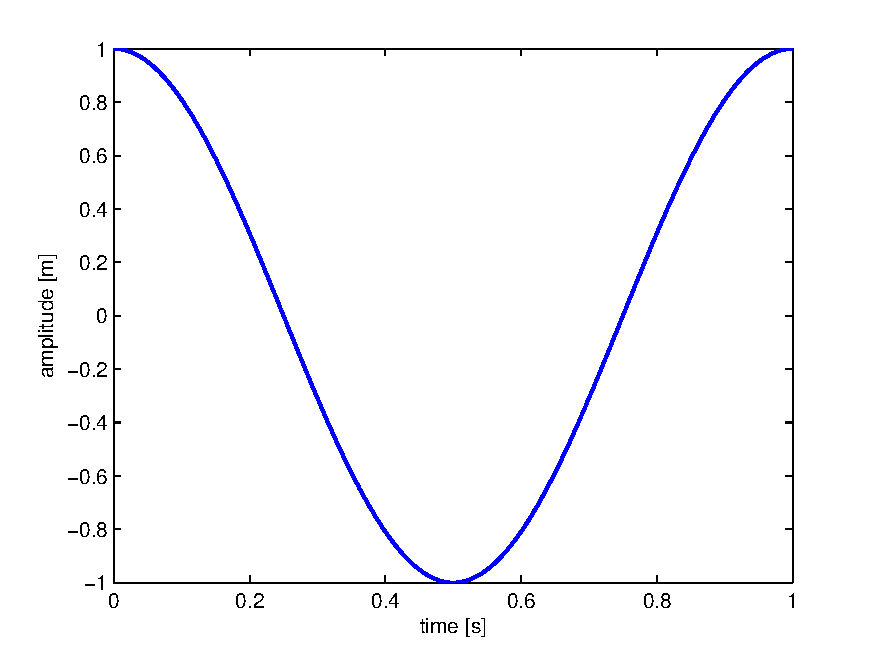
\includegraphics[width=\linewidth]{results}
% 	\caption{In-text Picture}
% 	\label{fig:results}
% \end{figure}

% Reference to Figure \ref{fig:results}.

% it depends
\subsection{Potential Issues}
%------------------------------------------------

\section{Industry Application Scenarios}

% \lipsum[10] % Dummy text

\subsection{Content Creation}

\subsubsection{Automatical Writing}
\paragraph{Case} Name % Dummy text
\subsubsection{Need-to-be-done}
\paragraph{Case} Name % Dummy text


\subsection{Chatbot}

\subsubsection{Customer Support}
\paragraph{Case} Name % Dummy text

\subsubsection{Q\&A Systems}
\paragraph{Case} Name % Dummy text

\subsection{Healcare}

\subsubsection{Diagnostic Assistance}
\paragraph{Case} Name % Dummy text

\subsubsection{Medical Record Generation}
\paragraph{Case} Name % Dummy text

\subsubsection{Health Analysis \& Advice}
\paragraph{Case} Name % Dummy text


\subsection{Education}

\subsubsection{Personalized Learning}
\paragraph{Case} Name % Dummy text

\subsubsection{Language Learning}
\paragraph{Case} Name % Dummy text

\subsubsection{Skills Training}
\paragraph{Case} Name % Dummy text

\subsection{Finace \& Legal}

\subsubsection{Sales and Marketing}
\paragraph{Case} Name % Dummy text

\subsubsection{Financial Analysis}
\paragraph{Case} Name % Dummy text

\subsubsection{Risk Assessment}
\paragraph{Case} Name % Dummy text

\subsubsection{Legal Assistance}
\paragraph{Case} Name % Dummy text


% \lipsum[11] % Dummy text

% \begin{table}[hbt]
% 	\caption{Table of Grades}
% 	\centering
% 	\begin{tabular}{llr}
% 		\toprule
% 		\multicolumn{2}{c}{Name} \\
% 		\cmidrule(r){1-2}
% 		First name & Last Name & Grade \\
% 		\midrule
% 		John & Doe & $7.5$ \\
% 		Richard & Miles & $2$ \\
% 		\bottomrule
% 	\end{tabular}
% 	\label{tab:label}
% \end{table}



% \lipsum[12] % Dummy text

% \begin{description}
% 	\item[Word] Definition
% 	\item[Concept] Explanation
% 	\item[Idea] Text
% \end{description}

% \subsubsection{Subsubsection}

% \lipsum[13] % Dummy text

% \begin{itemize}[noitemsep] % [noitemsep] removes whitespace between the items for a compact look
% 	\item First item in a list
% 	\item Second item in a list
% 	\item Third item in a list
% \end{itemize}

% \subsubsection{Subsubsection}

% \lipsum[14] % Dummy text

\section{Opportunities}

\subsection{Ehancing Efficiency}
\subsection{Improving Quality}
\subsection{Expanding Market Scale}
\subsection{Personalized Service}

\section{Challenges}

\subsection{Data Privacy}
\subsection{Data Resources}
\subsection{Ethics \& Bias}
\subsection{Costs}
\subsection{Regulatory \& Legal Risks}
\subsection{Technical Limitations}

\section{Conclusion}

%expectations, conclusions, suggestions, etc.
\lipsum[15-23] % Dummy text

%------------------------------------------------

\phantomsection
\section*{Acknowledgments} % The \section*{} command stops section numbering

\addcontentsline{toc}{section}{Acknowledgments} % Adds this section to the table of contents

So long and thanks for all the fish \cite{Figueredo:2009dg, Smith:2012qr}.

%----------------------------------------------------------------------------------------
%	REFERENCE LIST
%----------------------------------------------------------------------------------------

\phantomsection
\bibliographystyle{unsrt}
\bibliography{sample.bib}

%----------------------------------------------------------------------------------------

\end{document}